\chapter{Surfactantes}
\label{chp:tensoactivos}

\section{Introducción}
En el momento en que consideramos una dispersión fina de una fase dentro de otra, la interfase que delimita cada una de ellas se convierte en un tema de importancia. Esta relación se genera de manera natural debido a que la materia particulada posee una proporción mucho mayor de área superficial respecto a la masa. En la \autoref{fig:Area} se muestra este concepto, el área superficial de una esfera con radio de $1~cm$ ($4 \pi r^{2}$) es de aproximadamente $12~cm^{2}$, mientras que el área superficial de la misma cantidad de material pero en forma de esferas de diámetro de $1\mu$m es de $120000~cm^{2}$.
%The link between colloids and surfaces follows naturally from the fact %that particulate matter has a high surface area to mass ratio. The %surface area of a 1cm diameter sphere (4pr2) is 3.14cm2, whereas the %surface area of the same amount of material but in the form of 0.1mm %diameter spheres (i.e. the size of the particles in latex paint) is %314000cm2.
\begin{figure}
    \centering
    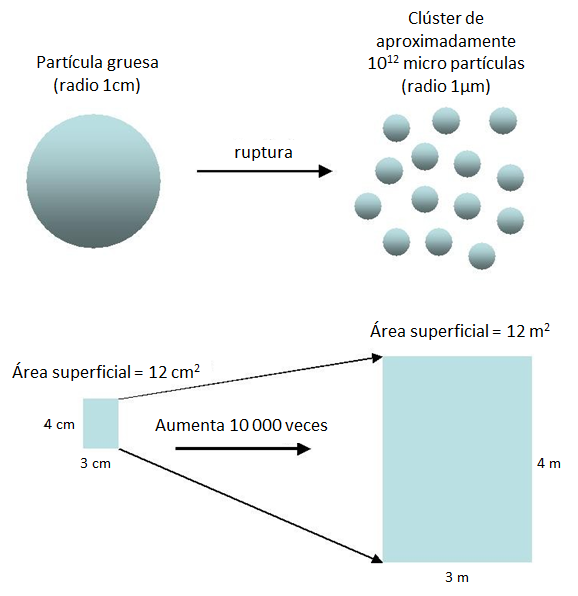
\includegraphics[width=0.7\textwidth]{Graphics/Area.png}
    \caption[Área superficial]{El área superficial de una esfera con radio de $1$cm ($4 \pi r^{2}$) es de aproximadamente $12 cm^{2}$ (como un cuadrilátero de $3 x 4$ cm), el mismo volumen ($4.2 cm^{3}$) puede ser ocupado por $10^{12}$ esferas de radio $1 \mu$m, con un área superficial de $12m^{3}$ (como un cuadrilátero de $3 x 4$ m). }
    \label{fig:Area}
\end{figure}

\subsection{Interfase}

\begin{description}
    \item [Definición] Para que dos fases existan en contacto una con otra, debe haber una región a través de la cual las propiedades intensivas del sistema pasen de las de una fase, a las de otra fase (\cite{Cosgrove}).
\end{description}
    
 Los términos \emph{superficial} e \emph{interfacial} se pueden encontrar intercambiados en la literatura, aunque rigurosamente tienen significados distintos. De manera general se puede decir que el término superficial se aplica en la región entre una fase condensada (líquido o sólido) y una fase gas o vacío, mientras que el término interfacial se aplica a sistemas que involucran dos fases condensadas.
 
 \subsection{Actividad Superficial}
 Algunas sustancias como los ácidos grasos y los alcoholes son solubles tanto en solventes como el agua y el aceite. La parte hidrocarburo de la molécula le concede la solubilidad en aceite, mientras el grupo polar, posee suficiente afinidad al agua, como para arrastrar consigo a una cadena corta de hidrocarburos no polar dentro de una solución acuosa.
 
 Estos materiales están formados de moléculas que cuando son disueltas en un solvente en bajas concentraciones, poseen la habilidad de adsorberse (o localizarse) en la interfase. Este comportamiento de adsorción es atribuido a la naturaleza del solvente y a la estructura química de la sustancia, que poseen un grupo polar y uno no polar en la misma molécula (ambifílicos).
 
 La fuerte adsorción de estos materiales en la interfase (o superficie) para formar una película monomolecular (o monocapa) es denominada como actividad superficial (\cite{Duncan}).
 
 \section{Surfactantes}
 
 Los materiales que presentan actividad superficial son denominados surfactantes o tensoactivos. En general los tensoactivos poseen una estructura química característica (ver \autoref{fig:Tenso}) que consiste de:
 
 \begin{itemize}
     \item Componente molecular de poca afinidad con la fase que lo rodea (por ejemplo el solvente) normalmente llamado el grupo liofóbico.
     \item  Unidades químicas que poseen una fuerte atracción hacia la fase que las rodea, denominadas el grupo liofílico.
 \end{itemize}

\begin{figure}
    \centering
    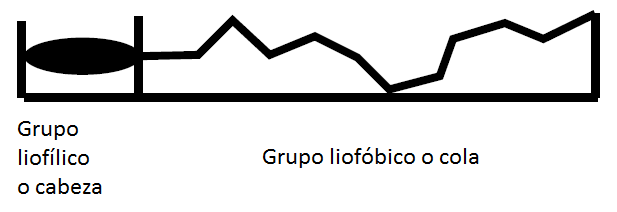
\includegraphics[width=0.9\textwidth]{Graphics/Tenso.png}
    \caption[Estructura de un tensoactivo]{La estructura básica de un material tensoactivo consiste de un grupo liofóbico que posee poca afinidad por el solvente y el grupo liofílico el cual presenta una fuerte interacción con el solvente. Adaptada de (\cite{Drew}). }
    \label{fig:Tenso}
\end{figure}


%Uno de los tipos de sistemas coloidales, clasificados como coloides de asociación (\autoref{chp:antescedentes}), son agregados de moléculas ambifílicas, que se asocian en un proceso impulsado dinámica y termodinámicamente, de manera que pueden ser soluciones a nivel molecular y sistemas coloidales simultáneamente.
%
%Los surfactantes son una importante y versátil clase de químicos. Debido a su naturaleza dual, están asociados con diversos fenómenos superficiales, por ejemplo la mojabilidad, y estos a su vez se encuentran en varios procesos industriales (\cite{Cosgrove}).

\subsection{Características de los surfactantes}

Debido a su naturaleza dual, los surfactantes se sitúan (adsorben) en la interfase de modo que su sección liofóbica (cola) se mantiene alejada de las fuertes interacciones con el solvente, mientras que la parte liofílica (cabeza) permanece en solución (\autoref{fig:adsorb}).

La adsorción esta asociada con un cambio energético dado que la energía libre de una molécula surfactante localizada en la interfase es menor que la de la misma molécula solubilizada en el seno de cualquiera de las fases. La acumulación de ambífilos en la interfase es un proceso espontáneo que resulta en la disminución de la tensión interfacial (o superficial). Este fenómeno ocurre con muchas otras sustancias como algunos alcoholes de media y larga cadena (ejemplo: n-hexanol, duodecanol), estos son sustancias que no son consideradas como surfactantes. 
Un surfactante se distingue por su capacidad de formar capas orientadas de moléculas en la interfase, y mas importante, formar estructuras autoensambladas (miscelas, vesículas) dentro del seno de las fases (\cite{Cosgrove}).

\begin{figure}
    \centering
    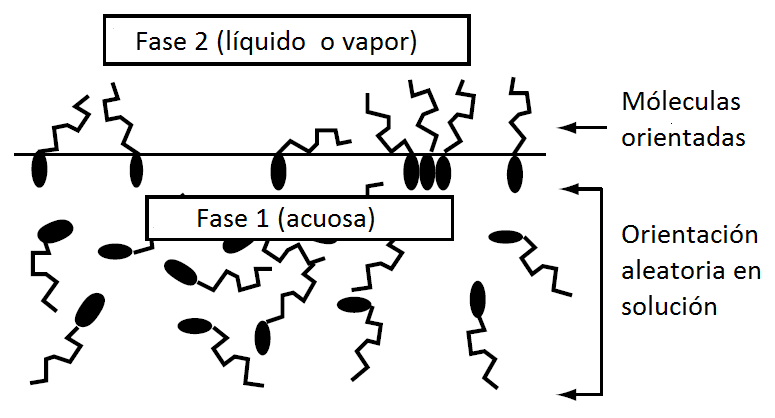
\includegraphics[width=0.9\textwidth]{Graphics/Adsorb.png}
    \caption[Adsorción en la interfase]{Cuando ocurre la adsorción en la interfase, las moléculas adsorbidas tienden a orientarse de manera que minimizan las interacciones no favorables entre la fase acuosa y las secciones de la molécula surfactante. Adaptada de (\cite{Drew}). }
    \label{fig:adsorb}
\end{figure}


\subsection{Clasificación}
Existen numerosas variaciones dentro de la estructura química de los grupos cola y cabeza de la molécula surfactante. El grupo cabeza puede tener carga o ser neutro, puede tratarse de una estructura pequeña y compacta o una cadena polimérica. El grupo cola normalmente es un hidrocarburo lineal o ramificado sencillo o doble, peor también puede ser un fluorocarbonado, un siloxano o contener grupos aromáticos. 

Dado que el solvente mas común e importante para los procesos industriales es el agua, comúnmente se describen a los surfactantes en función de sus grupos  hidrofílicos (cabezas) e hidrofóbicos (colas). Algunos de los grupos hidrofílicos e hidrofóbicos mas comunes se encuentran muestran en la \autoref{tab:surf1} y \autoref{tab:surf2}.

\begin{table}
 \caption[Grupos Hidrofílicos]{\raggedright Grupos hidrofílicos comúnmente encontrados en surfactantes comerciales (\cite{Cosgrove}).}
     \centering \footnotesize
     \begin{tabulary}{\textwidth}{L|L}
     \toprule 
        Clase & Estructura General\\ 
        \midrule              
        Sulfonato & $R-SO_{3^{-}}M^{+}$ \\
        Sulfato & $R-OSO_{3^{-}}M^{+}$ \\
        Carboxilato &  $R-COO^{-}M^{-}$ \\
        Fosfato & $R-OSO_{3^{-}}M^{+} $ \\
        Amonio & $R_{x}H_{y}N^{+}X^{-}$ \{$x=1-3, y=4-x$ \} \\
        Amonio cuaternario & $R_{4}N^{+}X^{-}$\\
        Betainos & $RN^{+}(CH_{3})_{2}CH_{2}COO^{-}$\\
        Sulfobetainos & $RN^{+}(CH_{3})_{2}CH_{2}CH_{2}SO_{3^{-}}$\\
        Polioxietileno & $R-OCH_{2}CH_{2}(OCH_{2}CH_{2})_{n}OH$\\
        Polioles & Sucrosa, sorbitan, glicerol, etilenglicol, etc.\\
        Polipéptidos & $R$-$NH$-$CHR$-$CO$-$NH$-$CHR'$-$CO$-...-$CO_{2}H$\\
        Poliglicidil & $R$-$(OCH_{2}CH[CH_{2}OH]CH_{2})_{n}$- ... -$OCH_{2}CH[CH_{2}OH$\\
     \midrule
     \bottomrule
     \end{tabulary}
     \label{tab:surf1}
\end{table}

\begin{table}
    \caption[Grupos Hidrofóbicos]{\raggedright Grupos hidrofóbicos comúnmente encontrados en surfactantes comerciales (\cite{Cosgrove}).}
    \centering \footnotesize
    \begin{tabulary}{\textwidth \tymin=99.73pt}{|L|L L|}
        \toprule 
        Grupo & Estructura general & ~\\ 
        \midrule              
        Alquilos & $CH_{3}(CH_{2})_{n}$ & n = $12$ - $18$\\
        Olefinas & {\scriptsize $CH_{3}(CH_{2})_{n}CH$=$CH_{2}$} & n = $7$ - $17$ \\
        %\multicolumn{3}{c}{~}\\ %%con esto dejamos una linea vacía
        Alquilbenzenos & \setatomsep{1em}\chemfig{[:0]CH_3{(}CH_2{)}_nCH_2-*6(=-=-=-)} & n = $6-10$, lineal o ramificado\\
        \multicolumn{3}{c}{~}\\ %con esto dejamos una linea vacía
        Alquilaromáticos & ~ & n = $1$ - $2$ soluble en agua ~~~~~ n = $8$ o $9$, soluble en aceite \\
        \multicolumn{3}{c}{~}\\ %con esto dejamos una linea vacía
        Alquilfenoles & \scriptsize\setatomsep{1em}\chemfig{[:0]CH_3{(}CH_2{)}_nCH_2-*6(=-=(-[,1.0]OH)-=-)} & n = $6-10$, lineal o ramificado\\
        \multicolumn{3}{c}{~}\\ %con esto dejamos una linea vacía
        Polioxipropilenos & ~ & n = grado oligomerización ~~~~~~~
        X = iniciador oligomérico \\
        \multicolumn{3}{c}{~}\\ %con esto dejamos una linea vacía
        Fluorocarbonados& $CF_{3}(CF_{2})_{n}COOH$ & n = $4-8$, lineal, ramificado o hidrogenado\\
        Siliconas & {\scriptsize\chemfig{CH_3O{(}SiO{)}_nCH_3}} & ~ \\
        \midrule
        \bottomrule
    \end{tabulary}
    \label{tab:surf2}
\end{table}

La clasificación mas útil para los agentes surfactantes se basa en la naturaleza del hidrófilo y los subgrupos se definen por la naturaleza del hidrófobo (\cite{Drew}). Los cuatro grandes grupos de surfactantes se definen como:

\begin{description}
    \item[Aniónicos] El grupo hidrofílico posee una carga negativa, como en el carboxil, sulfonatos y sulfatos.
    \item[Catiónicos] Con el hidrófilo exhibiendo una carga positiva, como por ejemplo en los haluros de amonio cuaternario.
    \item[No iónicos] Donde el hidrófilo no tiene carga pero debe su solubilidad en agua a grupos altamente polares como azúcares, polioxietileno o grupos similares.
    \item[Zwitteriónicos] También llamados \emph{anfóteros} son aquellos cuya molécula tiene o puede tener, una carga negativa y una positiva en su cadena principal (\autoref{fig:ZW1}).
\end{description}

%En química un zwitterion, palabra que proviene del alemán \textit{zwitter = híbrido}, es una molécula que posee carga positiva y negativa en diferentes puntos dentro de la molécula, pero que su carga neta es cero  (\autoref{fig:ZW1}). Los zwitteriones son llamados también \emph{sales internas}, iones \textit{amfolíticos o amfolitos (amfóteros)} (\cite{Dictionary:chem}). 


\begin{figure}
    \centering
    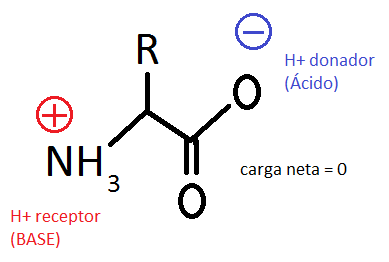
\includegraphics[width=0.7\textwidth]{Graphics/ZW3.png}
    \caption[Molécula zwitterion general]{En química un zwitterion, palabra que proviene del alemán \textit{zwitter = híbrido}, es una molécula que posee carga positiva y negativa en diferentes puntos dentro de la molécula, pero que su carga neta es cero. Los zwitteriones son llamados también \emph{sales internas}, iones \textit{amfolíticos o amfolitos (amfóteros)} (\cite{Dictionary:chem}).}
    \label{fig:ZW1}
\end{figure}

Debido a sus cargas eléctricas, un zwitterion será altamente soluble en agua y también soluble en solventes orgánicos. Las moléculas de agua son polares debido a la diferencia en cargas eléctricas entre las molécula de hidrógeno y oxígeno en el agua; esto es, los átomos de oxígeno del agua son atraídos por los cationes y los átomos de hidrógeno son atraídos por los aniones. Cuando un zwitterion es disuelto en agua, los átomos de hidrógeno rodean de manera inmediata el grupo negativamente cargado de la molécula zwitteriónica mientras que el los átomos de oxigeno del agua rodearan inmediatamente el grupo del zwitterion cargado positivamente, de este modo se logra una completa disolución en agua (\cite{Lenhinger:chem}).

\section{Propiedades de los surfactantes en solución}
Las soluciones de materiales con alta actividad superficial exhiben un comportamiento inusual en sus propiedades físicas. En soluciones diluidas un surfactante actúa como un soluto normal (como electrólito en el caso de un surfactante iónico). Sin embargo en ciertas concentraciones 
se presenta un cambio abrupto en varias propiedades físicas como la conductividad eléctrica, la presión osmótica, la turbidez y le tensión superficial (\autoref{fig:CMC}). El aumento de la presión osmótica con la concentración se vuelve anormalmente bajo y el aumento de la turbidez con la concentración se acelera.

\begin{figure}
    \centering
    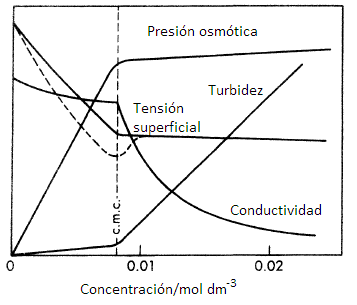
\includegraphics[width=0.9\textwidth]{Graphics/cmc.png}
    \caption[Concentracion micelar crítica]{La gráfica representa el cambio abrupto de las propiedades en la solución surfactante después de la concentración micelar crítica. Adaptada de (\cite{Duncan}). }
    \label{fig:CMC}
\end{figure}



Este comportamiento anómalo puede ser explicado en términos de la formación de agregados o micelas de iones surfactantes en los que las cadenas hidrocarbonadas lipofílicas se orientan hacia el interior de la micela, dejando al grupo hidrofílico en contacto con el medio acuoso (\autoref{fig:micela}) (\cite{McBain}). La concentración a partir de la cual la formación de micelas se vuelve apreciable se denomina \emph{concentración micelar crítica} (c.m.c). La micelación es un mecanismo alterno a la adsorción mediante el cual la energía interfacial de una solución surfactante decrece.

\begin{figure}
    \centering
    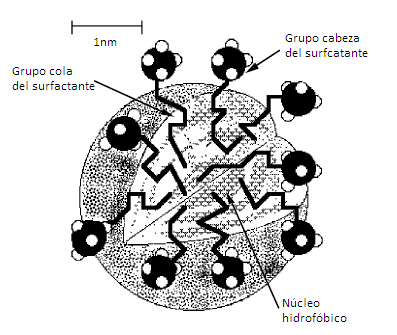
\includegraphics[width=0.9\textwidth]{Graphics/micela.png}
    \caption[Estructura general de una micela]{Representación de la estructura general de una micela. Adaptada de (\cite{Pashley}). }
    \label{fig:micela}
\end{figure}

La concentración micelar crítica puede ser determinada midiendo alguna propiedad física que se vea influenciada por la formación de estas estructuras contra la concentración de surfactante. En la práctica la tensión superficial y la conductividad eléctrica son las mas populares.

\section{Estructuras micelares}

\section{Estructuras supramoleculares}

La química supramolecular es la parte de la química encargada del estudio de los sistemas que involucran agregados de moléculas o de iones que se encuentran unidos por interacciones no covalentes, como lo son las interacciones electrostáticas, los puentes de hidrógeno  interacciones dipolo-dipolo (II-II interactions), interacciones de dispersión y efectos hidrofóbicos (\cite{IMP:Patente}).

La química supramolecular se puede dividir en dos grandes áreas:
\begin{itemize}
    \item Química de huésped - anfitrión.
    \item Química de autoensamble.
\end{itemize}

La diferencia entre ambas es una cuestión de tamaño y forma; cuando no existen diferencias significantes entre el tamaño y la forma de las especies y ninguna actúa como huésped de la otra, la unión no covalente entre dos o mas especies es referida como autoensamblaje.

Desde el punto de vista energético, las interacciones supramoleculares son mucho más débiles que las interacciones covalentes, que caen en el rango energético de entre $150$ y $450~KJ/mol ~$ pare enlaces sencillos. 
El rango energético de las interacciones no covalentes va de $2~KJ/mol$ para interacciones de dispersión hasta $300~KJ/mol$ para interacciones ión-ión (ver \autoref{tab:uspatent}). De manera que la suma de interacciones supramoleculares puede producir estructuras supramoleculares muy estables.

\begin{table}
\caption[Interacciones supramoleculares] {Rango energético de las interacciones supramoleculares. Adapta de \cite{IMP:Patente}.}
\centering
\begin{tabulary}{1.1\textwidth}{L |R}
    Interacción & Fuerza (KJ/mol) \\
    \toprule
    Ión-ión & $200-300$ \\
    Ión-dipólo & $50-200$ \\
    Dipólo-dipólo & $5-50$  \\
    Puente de hidrógeno & $4-120$ \\
    Cation - $\pi$ & $5-80$ \\
    $\pi$ - $\pi$ & $0-50$ \\
    Van der Waals & $<5$ \\
    \midrule
    \bottomrule
\end{tabulary}
\label{tab:uspatent}
\end{table}


% Supramolecular chemistry is the
% part of chemistry that takes care of the study of systems that
% involve molecules or ions aggregates that are bound through
% non-covalent interactions, such as electrostatic interactions,
% hydrogen bonds, II-II interactions, dispersion interactions
% and hydrophobic effects. Supramolecular chemistry can be
% divided in two large areas: 1) Host-Guest Chemistry and 2)
% Self-assembly. The difference between these two large areas
% is a matter of size and form; where there is no significant
% difference in size and none of the species acts as host to the
% other, the non-covalent bonding between two or more species
% is termed self-assembly.

% From the energetic point of view, supramolecular
% interactions are much weaker than covalent interactions,
% which fall in the energetic range of 150 to 450 K/mol for
% simple bonds. The non-covalent interactions energetic range
% goes from 2 kJ/mol for dispersion interactions to up to 300
% k/mol for ion-ion interactions (Table 1), and the sum of
% several Supramolecular interactions can produce highly
% stable Supramolecular complexes.

\begin{description}
    \item[Retículo] Según la \emph{IUPAC} \cite{IUPAC2} se trata de una región pequeña en un macromolécula en la cual al menos se forman cuatro cadenas formadas por reacciones o grupos de moléculas, o por interacciones entre moléculas existentes. Una región pequeña puede tratarse de un átomo, un grupo de átomos o un número de ramificaciones conectadas por enlaces, grupos de átomos o cadenas oligoméricas. En la mayoría de los casos un retículo es una estructura covalente sin embargo se utiliza también para describir interacciones químicas más débiles e incluso interacciones físicas.
\end{description}

Aquí iria la info de la India (\cite{NPTEL:Bio}).



\section{Reología}
\begin{description}
    \item[Reología] La reología es la rama
    \item[Reometría] La reometría es rama de la reología
\end{description}

Para introducir los conceptos básicos de reología hay que considerar un líquido contenido entre dos placas paralelas a cierta distancia \emph{h} como se muestra en la \autoref{fig:reo1}. La placa superior se desliza con una velocidad $v$ in la dirección \emph{x}, mientras que la placa inferior permanece estática. A velocidades suficientemente bajas para evitar la turbulencia, el fluido se moverá de manera uniforme y paralelo a las placas. Las velocidades locales $v_{x}$ varían de manera lineal en el espacio entre placas. En muchos casos las capas de fluido mas cercanas a las placas tienen la misma velocidad que la placa. De esta manera el gradiente $dv_{x}/{dy}$ de $v_{x}$ en la dirección \emph{y} es constante en todo el líquido.

\begin{figure}\centering
    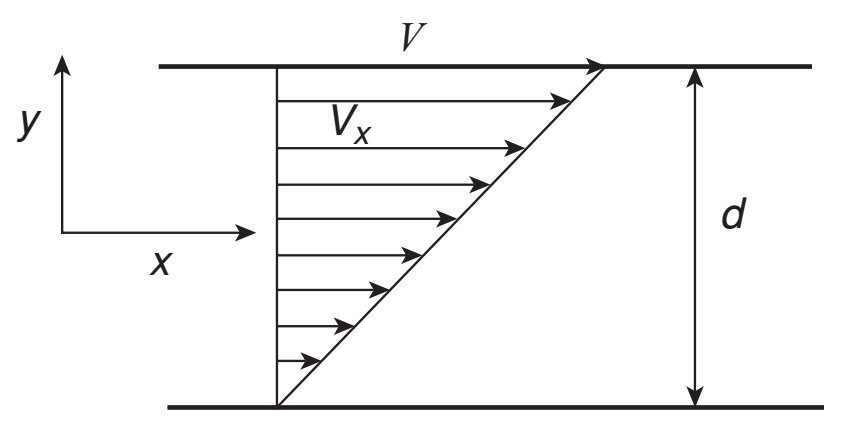
\includegraphics[width=0.7\textwidth]{Graphics/reo1.png}
    \caption[Flujo entre placas]{Flujo cortante entre dos placas, una fija y otra deslizante separadas por una distancia \emph{h}. Adaptada de ().}
    \label{fig:reo1}
\end{figure}

\begin{equation}
\frac{dv_{x}}{dy}= \frac{V}{h}=\dot{\gamma}=constante
\end{equation}

Para generar el flujo se necesita aplicar una fuerza \emph{$F_{xy}$} a la placa superior. El primer subíndice \emph{x} especifica la dirección en la cual se aplica la fuerza mientras el segundo \emph{y}, define el plano al cual se le aplica la fuerza en términos de la normal del plano. La fuerza requerida para mover la placa superior a una velocidad $v$ es proporcional al área superficial de las placas. Por lo anterior, la característica que es relevante en la dinámica involucrada es la fuerza por unidad de área o esfuerzo, $\sigma_{xy}$. Este esfuerzo de corte es trasmitido de una placa a otra y actúa sobre cada elemento del fluido entre ellas. El factor cinético que determina el nivel de los esfuerzos internos, en este caso es el gradiente de velocidad o velocidad de corte. Para fluidos con baja concentración molar, la ecuación constitutiva de Newton para la viscosidad puede ser aplicada. Esta relación especifica, en términos simples, que el esfuerzo es proporcional al gradiente de velocidad. La constante de proporcionalidad, es el coeficiente de viscosidad $\eta$, que expresa la resistencia al flujo para \emph{Fluidos Newtonianos}.

\begin{equation}
\sigma_{xy}=\eta \frac{dv_{x}}{dy}
\end{equation}

La \emph{Ley de Newton} es el ejemplo mas simple de una ecuación constitutiva de reología. Esta expresa la relación intrínseca entre esfuerzos y la cinética para un fluido. Se puede combinar con las leyes de conservación de masa, momento y energía para resolver varios problemas de flujo.

\subsection{Cinemática}
Los flujos no son siempre sencillos como en el caso de la \autoref{fig:reo1}. En términos generales la velocidad no se encuentra necesariamente orientada a lo largo de una linea coordenada. Esta debe ser descrita por un campo de vectores $v$(r) en el cual la velocidad $v$ para cada posición r(x,~y~,z) tiene componentes en las direcciones coordenadas ($v_{x},v_{y},v_{z}$). En la figura anterior solamente una componente de la velocidad diferente de cero varia en solo una dirección coordenada. En general para flujo en tres dimensiones, cualquier gradiente de cualquier componente puede ser diferente de cero. Por lo tanto el gradiente de velocidad debe ser representado por una matriz $\nabla v$:

\begin{equation} 
\nabla v = \left( 
\begin{matrix} 
\delta v_{x}/\delta{x} & \delta v_{x}/\delta{y} & \delta v_{x}/\delta{z} \\
\delta v_{y}/\delta{x} & \delta v_{y}/\delta{y} & \delta v_{y}/\delta{z} \\
\delta v_{z}/\delta{x} & \delta v_{z}/\delta{y} & \delta v_{z}/\delta{z} 
\end{matrix} \right)
\end{equation}

Para el caso de un flujo cortante en una sola dimensión usando coordenadas cartesianas, por convención \emph{x} (ó $1$) es la dirección de flujo, \emph{y} (ó $2$) es la dirección del gradiente, y \emph{z} (ó 3) la dirección neutral o de vorticidad. Las componentes de la matriz en la ecuación (30) representan entidades físicas y por lo tanto obedecen a ciertas reglas de transformación para los componentes o tensores (o transformaciones lineales). Lo mismo aplica para las componentes de esfuerzo.

El vector $v$ y el tensor $\nabla v$ pueden contener componentes diferentes de cero aun cuando no exista el flujo. Este caso, por ejemplo, se presenta cuando un líquido rota como un cuerpo solido sin algún flujo. Lo anterior hace que el gradiente de velocidad no sea adecuado para describir la cinemática en una ecuación constitutiva. Este inconveniente se evita utilizando la parte simétrica del gradiente de velocidad, que no se ve afectada por la rotación como cuerpo sólido. Esto resulta en el tensor de tasa de deformación, \textbf{D}, con componentes:

\begin{equation}\Large
D_{ij} = \left(
\begin{matrix}
%
\frac{\delta v_{x}}{\delta{x}} & \frac{1}{2}(\frac{\delta v_{x}}{\delta{y}}+\frac{\delta v_{y}}{\delta{x}}) & \frac{1}{2}(\frac{\delta v_{x}}{\delta{z}}+\frac{\delta v_{z}}{\delta{x}}) \\
%
\frac{1}{2}(\frac{\delta v_{y}}{\delta{x}}+\frac{\delta v_{x}}{\delta{y}}) & \frac{\delta v_{y}}{\delta{y}} & \frac{1}{2}(\frac{\delta v_{y}}{\delta{z}}+\frac{\delta v_{z}}{\delta{y}}) \\
%
\frac{1}{2}(\frac{\delta v_{z}}{\delta{x}}+\frac{\delta v_{x}}{\delta{z}}) & \frac{1}{2}(\frac{\delta v_{z}}{\delta{y}}+\frac{\delta v_{y}}{\delta{z}}) & \frac{\delta v_{z}}{\delta{z}}
\end{matrix}
\right)
\end{equation}

Aplicado para el caso de flujo presentado en la \autoref{fig:reo1}, esto hace que la ecuación (29) cambie a $\sigma_{xy}=2\eta D_{xy}$. Para evitar arrastrar el factor de $2$, a menudo se utiliza el tensor $\dot{\gamma}$, definido como $2D$. Dado que la matriz de la ecuación (31) es simétrica respecto de su diagonal principal, la suma de los términos en la diagonal expresa la tasa a la cual cambia el volumen. En la mayoría de los casos de flujo en líquidos, se asume que el volumen permanece constante durante el flujo (flujo incompresible), lo que requiere que este término sea cero:

\begin{equation}
\nabla * v = \frac{\delta v_{x}}{\delta_{x}}+\frac{\delta v_{y}}{\delta_{y}}+\frac{\delta v_{z}}{\delta_{z}}=0
\end{equation}
Cuando existen términos diferentes de cero en la diagonal principal de \textbf{D} ($D_{ij},i \neq j$) estos describen un movimiento cortante en el cual las capas del fluido deslizan una sobre de otra. Para flujo en una sola dimensión, esto se reduce a un simple flujo cortante, caracterizado por el esfuerzo de corte $2D_{xy}$ ó $\dot{\gamma}$. Por otra parte cuando solo las componentes de la diagonal principal ($D_{ij},i=j$) son diferentes de cero, estas describen un movimiento en el cual el fluido no es cortado si no estirado o comprimido a lo largo de las lineas coordenadas. El caso mas simple de este fenómeno es el de estiramiento uniaxial \autoref{fig:reo2}. La aceleración en $x$ (ó 1) causa un flujo en las direcciones cruzadas en orden de satisfacer la conservación de masa expresada en la ecuación:

\begin{figure}\centering
    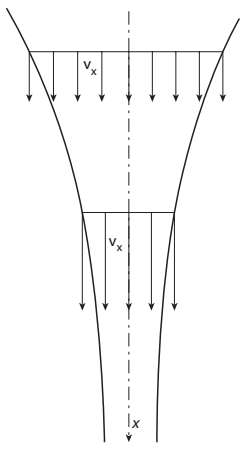
\includegraphics[width=0.4\textwidth]{Graphics/reo2.png}
    \caption[Flujo extensional uniaxial]{Flujo extensional uniaxial. Un material viscoso es estirado por una fuerza que actúa a lo largo de la dirección $x$. Adaptada de ().}
    \label{fig:reo2}
\end{figure}

\begin{equation}
\frac{\delta v_{y}}{\delta_{y}}=\frac{\delta v_{z}}{\delta_{z}}= -\frac{1}{2} \frac{\delta v_{x}}{\delta_{x}}
\end{equation}

Las componentes fuera de la diagonal principal son todas cero. Las velocidades en las direcciones $y$ y $z$ son idénticas por razones de simetría.
En casos de flujo mas complejos, ambas, las componentes de corte y extensionales pueden estar presentes. Por ejemplo en flujos convergentes, cuando un líquido fluye a través de una reducción. La fricción en la pared causa el corte, mientras que la reducción obliga al fluido a acelerarse para permitir que la misma cantidad de materia fluya a través de las secciones transversales. Esto induce una componente extensional.

\subsection{Dinámica}
Así como es necesario generalizar el gradiente de velocidad (ecuación 28) al tensor de tasa de deformación (ecuación 31), se debe adaptar la expresión del esfuerzo de corte para aplicarlo a casos mas generales de flujo. En el caso de flujo cortante simple, solo la componente del esfuerzo $\sigma_{xy}$ es considerada. La \autoref{fig:reo3} muestra un paralelepípedo alrededor de un punto en el seno del fluido, con sus lados paralelos a las planos coordenados. Los planos son identificados por su dirección normal al plano.

\begin{figure}\centering
    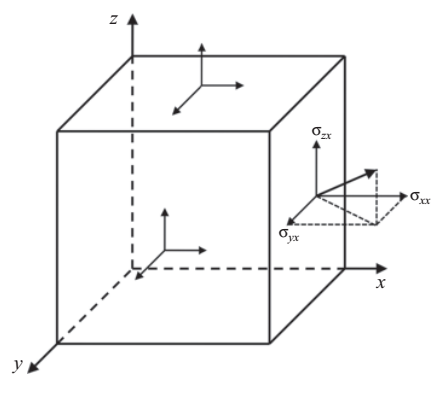
\includegraphics[width=0.7\textwidth]{Graphics/reo3.png}
    \caption[Componentes del esfuerzo de corte]{Componentes del esfuerzo de corte $\sigma$. Adaptada de ().}
    \label{fig:reo3}
\end{figure}

La fuerza $F_{i}$, sobre un plano arbitrario $A_{i}$ en el material, no está orientada de manera perpendicular ni paralela al plano. Dicha fuerza, o su correspondiente esfuerzo, en general se descompone en tres componentes. Para el plano $dA_{x}=d_{y}d_{z}$ perpendicular a la dirección $x$, las componentes dadas por el cociente $dF_{x}/dydz$ del esfuerzo son $\sigma_{xx},\sigma_{yx},\sigma_{zx}$ (\autoref{fig:reo3}). El primer subíndice se refiere a la dirección de la componente de esfuerzo mientras que el segundo se refiere a la normal al plano sobre la cual actúa el esfuerzo. Aplicando el mismo procedimiento al los esfuerzos en los demás planos coordenados, resulta en la matriz de componentes del esfuerzo $\sigma_{ij}$:

\begin{equation}
\sigma_{ij}=\left( \begin{matrix}
\sigma_{xx} & \sigma_{xy} & \sigma_{xz} \\
\sigma_{yx} & \sigma_{yy} & \sigma_{yz} \\
\sigma_{zx} & \sigma_{zx} & \sigma_{zz}
\end{matrix} \right)
\end{equation}

Se puede demostrar que los esfuerzos en cualquier plano de orientación arbitraria en un punto dado, pueden ser calculados a partir de las nueve componentes de esfuerzo sobre los planos coordenados. Los esfuerzos pueden ser expresados en varios sistemas de coordenadas, siguiendo ciertas reglas de transformación, como en el caso del gradiente de velociada y por lo tanto describen un tensor \textbf{$\sigma$}.

Así como con el tensor de tasa de deformación, se distinguen dos diferentes componentes del tensor de esfuerzo. Las componentes en la diagonal principal, $\sigma_{ii}$, están orientadas de manera normal al plano sobre el que actúan; estos son los \emph{esfuerzos normales}. Las componentes fuera de la diagonal principal, se encuentran orientados según el plano a considerar; estos son los \emph{esfuerzos de corte}. Para fluidos ordinarios se puede demostrar que la matriz de esfuerzos $\sigma_{ij}$ es simétrica con respecto a su diagonal principal (igual que el tensor de tasa de deformación).

\begin{equation}
\sigma_{ij}=\sigma_{ji}
\end{equation}

Aun cuando no existe flujo, existe una presión hidrostática en el fluido. Esto origina una presión idéntica (esfuerzo normal) en todas direcciones, mientras que los esfuerzos de corte son todos cero:

\begin{equation}
\sigma_{ij}= \left( \begin{matrix}
-P & 0 & 0 \\
0 & -P & 0 \\
0 & 0 & -P
\end{matrix} \right) = -P\left( \begin{matrix}
1&0&0 \\
0&1&0 \\
0&0&1
\end{matrix} \right)
\end{equation}

Por convención la presión es negativa y el tensor positivo. La matriz de la derecha representa el tensor unitario \textbf{I}, el cual se escribe en notación vectorial como:

\begin{equation}
\sigma=-PI
\end{equation}

La aplicación de un flujo cortante a un fluido newtoniano, resulta en esfuerzos de corte proporcionales al la velocidad de corte (gradiente de velocidad). En términos de tensores, la expresión para la ecuación constitutiva de Newton es:
\begin{equation}
\sigma = -PI+2\eta D
\end{equation}

en donde el \emph{esfuerzo extra} $\sigma +P\textbf{I}$ es el factor de relevancia para la reología dado que la presión no afecta el flujo de fluidos incompresibles. Las componentes normales del esfuerzo extra son siempre cero para fluidos newtonianos. La cantidad de energía (por unidad de volumen) requerida para el caso simple de flujo cortante en un fluido newtoniano es $\sigma : D=\eta \dot{\gamma^{2}}$ que se disipa como flujo de calor.

\subsection{Fluidos Newtonianos Generalizados}
Para la mayoria de las suspensiones, el esfuerzo de corte sn flujo cortante simple, no es proporcional a la velocidad de corte y por ello no satisfacen la ley de Newton; estos son \emph{no newtonianos}.

Como primer caso de fluido no newtoniano están aquellos para los cuales el esfuerzo de corte está determinado en todo momento por un valor instantáneo de velocidad de corte, pero que no es proporcional. Los fluidos de este tipo son \emph{fluidos newtonianos generalizados}. En este caso la viscosidad es definida como \emph{viscosidad aparente} puesto que es función de la velocidad de corte. La \autoref{fig:reo4} muestra las formas posibles de la función $\sigma(\dot{\gamma})$

\begin{figure}\centering
    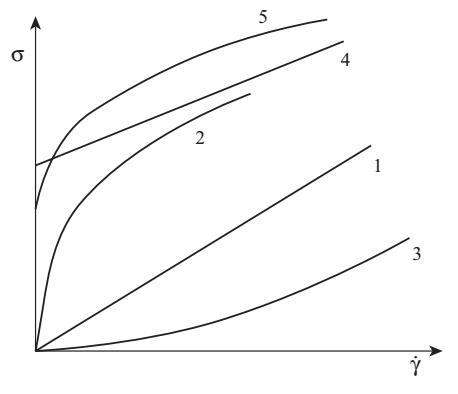
\includegraphics[width=0.7\textwidth]{Graphics/reo4.png}
    \caption[Curvas reológicas generales]{Curvas generales de esfuerzo de corte vs velocidad de corte. (1) Newtoniano; (2) Adelgazante; (4) Espesante; (5) Materiales con esfuerzo de cedencia Adaptada de ().}
    \label{fig:reo4}
\end{figure}

La curva (1) representa el caso newtoniano. En la curva (2) el esfuerzo de corte se incrementa por debajo de la proporciónal a la velocidad de corte, de manera que la viscosidad, (el cociente entre ambos) decrece con el incremento en la velocidad de corte. Este comportamiento describe un adelgazamiento al corte. El caso opuesto es la curva (3), donde la viscosidad se incrementa con el aumento de la velocidad de corte, \emph{Engrosamiento al corte}. Algunas sustancias pueden presentar ambos comportamientos dependiendo de la región de velocidad de corte en la que se encuentran.

Las curvas (2) y (3) representan relaciones no lineales entre el esfuerzo de corte y la velocidad de corte, pero al ser graficados de manera logarítmica se ajustan a una línea recta, lo que significa que esta relación se puede describir con una ley de potencias:

\begin{equation}
\sigma = k\dot{\gamma^{n}}
\end{equation}

donde $n$ el índice de ley de potencias, es la pendiente de la recta en una gráfica logarítmica.

De manera que la ecuación constitutiva de Newton para fluidos de este tipo es conocida como ley de potencias, donde para $n<<1$ se describe un adelgazamiento y $n>1$ describe un engrosamiento. La viscosidad en un fluido ley de potencias cambia de manera proporcional a $\dot{\gamma^{n-1}}$. Para $n<1$, la viscosidad se incrementa indefinidamente ($\eta_{\infty}$) a medida que la velocidad de corte tiende a cero, y por el contrario la característica asintótica de la curva hace que para velocidades de corte altas la viscosidad tiende a cero ($\eta_{0}$), de manera que estas curvas de viscosidad se describen mediante el modelo de viscosidad de \emph{Cross} (REF 27):

\begin{equation}
\eta-\eta_{\infty}=\frac{\eta_{0}-\eta_{\infty}}{1+(k^{'}\dot{\gamma})^{m}}
\end{equation}

Para fluidos cuyo comportamiento se puede describir mediante las ecuaciones (39) y (40) el esfuerzo de corte disminuye hacia cero a medida que la velocidad de corte tiende a cero, pero siempre debe existir una velocidad de corte diferente de cero, para producir un esfuerzo de corte diferente de cero. De manera que el fluido no puede existir en equilibrio bajo un esfuerzo de corte diferente de cero.

Algunos materiales exhiben un valor de esfuerzo de corte finito y diferente de cero, cuando la velocidad de corte es disminuida sistemáticamente, como en el caso de las curvas (4) y (5) en la \autoref{fig:reo4}. Mientras que para valores de velocidad de corte altos aún presentan un comportamiento newtoniano. La curva (4) describe un \emph{cuerpo de Bingham}:

\begin{equation}
\sigma = \sigma^{B}_{y} + \eta_{pl}\dot{\gamma}
\end{equation}

donde las características de del material son el esfuerzo de cedencia de Bingham $\sigma^{B}_{y}$ y la viscosidad plástica $\eta_{pl}$. Cuando el límite superior de velocidad de corte describe una ley de potencias, mas que un comportamiento newtoniano, se puede utilizar el modelo de \emph{Herschel-Bulkley}:

\begin{equation}\centering
\sigma= \sigma^{H}_{y}+k\dot{\gamma^{n}}
\end{equation}

%Adicionalmente existe un tercer modelo usado con frecuencia para describir a las supensiones con esfuerzo de cedencia:
%\begin{equation}
%\sigma^{n}=\sigma^{n}_{y}+k\dot{\gamma^{n}}
%\end{equation}
%cuando $n=1/2$ esta se convierte en la ecuación de \emph{Casson}, que es un modelo utilizado para describir el flujo sanguineo.

Adicional al esfuerzo de cedencia algunas suspensiones presentan otra complicación, la viscosidad no es solo función del la velocidad de corte instantánea, si no que la agitación o el corte ocasionan una disminución gradual en la viscosidad, la cual se recupera cuando el material esta en reposo. Una viscosidad dependiente del tiempo pero reversible define el concepto de \emph{tixotropía}. 

\subsection{Viscoelasticidad}

Los materiales \emph{viscoelásticos} combinan las propiedades elásticas de los sólidos con las de los fluidos viscosos. Los esfuerzos en un cuerpo elástico dependen de que tan grande es la desviación en la forma actual del cuerpo, de su forma original no deformada ni sometida a esfuerzo alguno, independientemente de la escala de tiempo de la deformación. Siempre que un esfuerzo haya sido aplicado, incluso por un largo tiempo, un material elástico siempre regresa a su estado no deformado cuando los esfuerzos son retirados. De manera ideal un material elástico tiene una perfecta "memoria" para regresar a su configuración no deformada. Un líquido, por otro lado, no posee esta memoria, de modo que aún cuando el esfuerzo de corte es retirado el fluido permanece en la última posición alcanzada.

Al aplicar de manera repentina una deformación de corte y mantenerla constante, en un sólido elástico el esfuerzo resultante permanecerá constante de manera indefinida. En un líquido el esfuerzo será muy alto cuando la deformación es aplicada de manera rápida, pues la velocidad de corte sera muy alta, pero una vez que termina la rápida deformación, no habrá flujo y el esfuerzo caerá inmediatamente a cero. Por otra parte en un material viscoelástico, el esfuerzo al corte disminuirá gradualmente en el tiempo, este fenómeno es conocido como \emph{relajación del esfuerzo}. Si el material viscoelástico es un sólido el esfuerzo se relajará parcialmente hasta un valor finito, mientras que si se trata de un líquido el esfuerzo se relaja hasta el valor de cero. 

Si retomamos el caso de flujo cortante de la figura \autoref{fig:reo1}, pero ahora en lugar de de moverse con una velocidad constante,la placa superior ejerce un movimiento sinusoidal $X_{p}(t) = X_{p,0}~seno(\omega t)$, donde $X_{p,0}$ pico máximo del desplazamiento. Esto genera una deformación dependiente del tiempo $\gamma(t)$ (linea continua en la 
\autoref{fig:reo5})

\begin{figure}
    \centering
    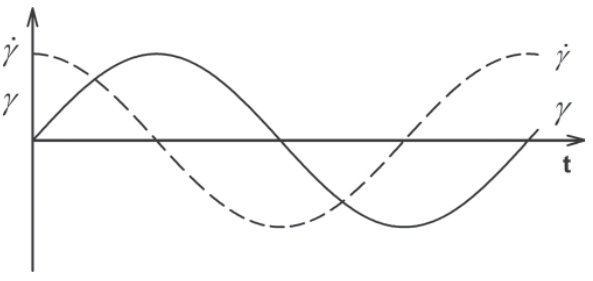
\includegraphics[width=0.8\textwidth]{Graphics/Reo5.png}
    \caption[Deformación en flujo oscilatorio]{Deformación, dependiente del tiempo, generada por una placa que ejerce un movimiento sinusoidal. Adaptada de ().}
    \label{fig:reo5}
\end{figure}
%
%
%
%
%
%    E            S             P           A           C          I         O
%
%
%
%
\subsection{Geles}
%Ejemplo del slim     alcohol polivinilico + tetraborato de sodio interacciones moleculares quimica supramolecular fuerzas de londo, ion dipolo, 
%PLATEAU:a state of little or no change following a period of activity or progress.
\begin{description}
\item[Definición] En términos generales un gel puede ser definido como un estado intermedio de la materia entre el comportamiento reológico de sólido y el de un líquido. Consiste de una fase dispersa (polímero o coloide) y un medio de dispersión (agua u otro solvente), y puede ser muy semejante a un líquido o a un sólido. Su característica líquida se debe a que el mayor constituyente es el solvente. Su comportamiento de sólido proviene de la red formada por retículos que impide que el gel fluya y se caracteriza por tener un módulo elástico finito (\cite{Nishinari2009}).
%\item[Retículo] Según la \emph{IUPAC} \cite{IUPAC2} se trata de una región pequeña en un macromolécula en la cual al menos se forman cuatro cadenas formadas por reacciones o grupos de moléculas, o por interacciones entre moléculas existentes. Una región pequeña puede tratarse de un átomo, un grupo de átomos o un número de ramificaciones conectadas por enlaces, grupos de átomos o cadenas oligoméricas. En la mayoría de los casos un retículo es una estructura covalente sin embargo se utiliza también para describir interacciones químicas más débiles e incluso interacciones físicas.
\end{description}


Un gel puede ser definido de manera reológica o de manera estructural, En términos de su reología, un gel es un sistema que no fluye y que puede ser caracterizado por la presencia en su reograma de una zona meseta del módulo de almacenamiento y una valor de $tan(\delta) < 0.1$ en un rango de frecuencia angular de $10^{-3}~a~10^{2}~~rad/s$. Estructuralmente un gel es definido por la conectividad del sistema. Un gel en un sistema que consiste de moléculas, partículas, cadenas, etc. que está parcialmente conectadas una con otra por retículos a escala macroscópica.

\subsubsection{Clasificación reológica}
Dado que este trabajo hace hincapié en la definición reológica de gel, es importante mencionar que algunos autores han clasificado el comportamiento reológico de los geles en cuatro grandes grupos de acuerdo con su espectro mecánico, la dependencia del modulo de almacenamiento y el modulo de pérdida (\emph{G' y G''} respectivamente) con la frecuencia, en un rango aceptablemente accesible a la tecnología comercial de entre $10^{-3}~a~ 10^{2}~~rad/s$ (\cite{Clark}).

\begin{itemize}
    \item 1. Gel Fuerte (gel elástico o verdadero). \emph{G'} es mucho más grande que \emph{G''} y ambos módulos son independientes de la frecuencia.
    \item 2. Gel débil (líquido estructurado). \emph{G'} ligeramente más grande que \emph{G''} y ambos módulos son ligeramente dependientes de la frecuencia.
    \item 3. Polímero entrecruzado. \emph{G'} es más pequeño que \emph{G''} para frecuencias mas bajas, pero ambos módulos se incrementan con el incremento de frecuencia y muestran un cruce luego del cual \emph{G'} se vuelve más grande que \emph{G''} para frecuencias mas altas.
    \item 4. Polímero no entrecruzado. \emph{G'} es mucho más pequeño que \emph{G''} para cualquier frecuencia y ambos módulos son fuertemente dependientes de la frecuencia.
\end{itemize}

El reograma típico para un líquido estructurado se muestra en la \autoref{fig:estructurado}.

\begin{figure}\centering
    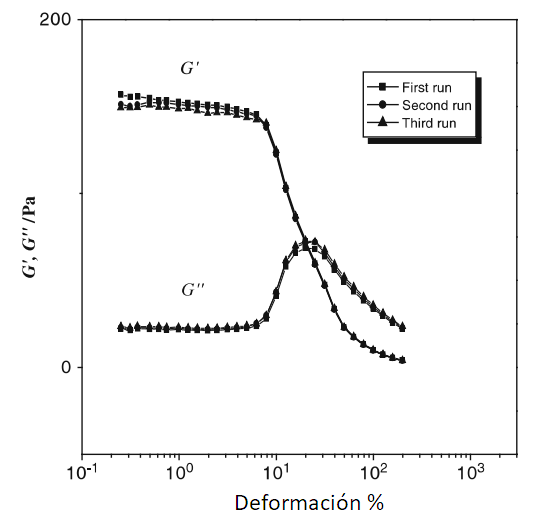
\includegraphics[width=0.9\textwidth]{Graphics/weak_gel}
    \caption[Reograma de un gel débil.]{Dependencia de los módulos de almacenamiento \emph{G'} y pérdida \emph{G''} con la deformación. Reograma típico de un gel débil o fluido estructurado. Obtenido mediante un barrido de deformación con una frecuencia angular de 1 rad/s. Ejemplo de una solución acuosa de SPG-sorbitol. Adaptada de (\cite{Nishinari2009})}
    \label{fig:estructurado}
\end{figure}

\subsubsection{Temperature Dependence}
To study this issue further, rheological characterization and viscosity analysis arepresented. A thermorheological simplefluid allows for the use of the superposition of the effects of the time and temperature, which we can associate just to the increment in kinetic energy.
In simplefluids, other mechanisms, such as phase change, structural rearrangement, and segregation, among other phenomena, are not present.

As mentioned before, to measure the shear viscosity, a simple velocity gradient is required; in the region of low shear rates, the fluids tend to behave as Newtonian, and this defines the “zero-shear viscosity”. The most commonly used model to correlate the temperature dependence of the viscosity of a fluid is the Arrhenius equation:

\begin{equation}\centering
\eta(T) = A~\exp{ \frac{E_{a}}{RT} } 
\end{equation}

in which $\eta$ is the viscosity, $T$ is the absolute temperature, $A$ is a material constant, $E_{a}$ is the fluid-dependent activation energy, and $R$ is the universal gas constant.

in which $\eta$ is the viscosity (in units of $Pa*s$), $T$ the temperature (in Kelvin), $A$ a constant, $E_{a}$ the fluid-dependent activation energy (in units of $J~mol^{-1}$), and $R$ the universal gas constant (in units of $J~K^{-1} mol^{-1}$).